\documentclass{beamer}

\usetheme{MagdeburgFIN}
\usefonttheme{structurebold}
\usepackage{graphicx}
\usepackage{float}
\usepackage{url}
\usepackage{pdfpages}
\usepackage{array}
\newcolumntype{M}[1]{>{\centering\arraybackslash}m{#1}}


\title{Adaptive Indexing: between Lazy but Lightweight Cracking and Eager but Expensive Merging}
\author{Pavlo Shevchenko}
\date{July 13, 2017}
\institute{Seminar on Modern Software Engineering and Database Concepts}

\begin{document}

\begin{frame}[plain]
 \titlepage
\end{frame}

\begin{frame}
\frametitle{Table of Contents}
\tableofcontents
\end{frame}

\section{Overview of Indexing}
\begin{frame}
\frametitle{Overview of Indexing}
\textbf{Database Indexes:}
\begin{itemize}
\item{help to decrease the query response time;}
\item{structure optimized for search with references to original entries;}
\item{precalculated before the first query arrives (\emph{offline indexing});}
\item{used to be stored on disk in the form of B-Trees.}
\end{itemize}
\pause
\textbf{Issues:}
\begin{itemize}
\item{in-memory databases $\Rightarrow$ more lightweight structures;}\pause
\item{growing amounts of data $\Rightarrow$ larger indexes;} \pause
\item{sophisticated queries $\Rightarrow$ many indexes;} \pause
\item{unpredictable behavior of users $\Rightarrow$ hard to predicate an attribute.}
\end{itemize}
\end{frame}

\section{Definition of Adaptive Indexing}
\begin{frame}
\frametitle{Definition of Adaptive Indexing}
\textbf{Core Idea:}
\begin{itemize}
\item{automated maintenance and tuning of indexes by DBMS;}
\item{continuous reorganization of the physical design during incremental \emph{online indexing}.}
\end{itemize}
\end{frame}

\section{Goal}
\begin{frame}
\frametitle{Research Goal}
\pause
Study the \emph{evolution} of adaptive indexing: \pause
\begin{itemize}
\item{\textbf{Past:}} Origin of adaptive indexing. \pause
\item{\textbf{Present:}} Current approaches for adaptive indexing. \pause
\item{\textbf{Future:}} Unresolved questions regarding adaptive indexing.
\end{itemize}
\end{frame}

\section{Background}
\begin{frame}
\frametitle{Background. Partial Index}
\begin{figure}
\centering
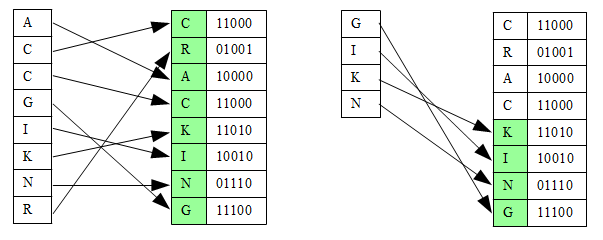
\includegraphics[width=\textwidth]{graphics/partial.png}
\caption{Full Index and Partial Index [1]}
\end{figure}
\end{frame}

\begin{frame}
\frametitle{Background. Soft Index}
In contrast to \emph{hard indexes}, which are created and managed by DBA, \emph{soft indexes} are created, modified and dropped by a DBMS [2].\\ \pause
\vspace{0.5cm}\textbf{Workflow:} \pause
\begin{enumerate}
\item{Collect information about the current state of a system.} \pause
\item{Analyze this information and choose index candidates for  materialization.} \pause
\item{Create or drop some indexes based on this analysis.}
\end{enumerate}
\end{frame}

\section{Adaptive Indexing}
\begin{frame}
\frametitle{Approaches for Adaptive Indexing}
\textbf{Goal:} provide fast access to the data and the self-organized behavior of a database system. \pause
\begin{enumerate}
\item{Database Cracking [3]:}
\begin{itemize}
\item{index maintenance is a byproduct of query processing;}
\item{continuous physical reorganization (\textit{cracking} database into manageable pieces).}
\end{itemize}
\pause
\item{Adaptive Merging [4]:}
\begin{itemize}
\item{adaptive nature of cracking;}
\item{better query response time and quicker adaption.}
\end{itemize}
\pause
\item{Hybrid Approaches [5]:}
\begin{itemize}
\item{combine strength of \emph{database cracking} and \emph{adaptive merging}.}
\end{itemize}
\end{enumerate}
\end{frame}

\subsection{Database Cracking}
\begin{frame}
\frametitle{Database Cracking}
\textbf{Main Idea: } incrementally perform quicksort on a copy of a column using crack-in-three or crack-in-two. \pause
\begin{figure}
\centering
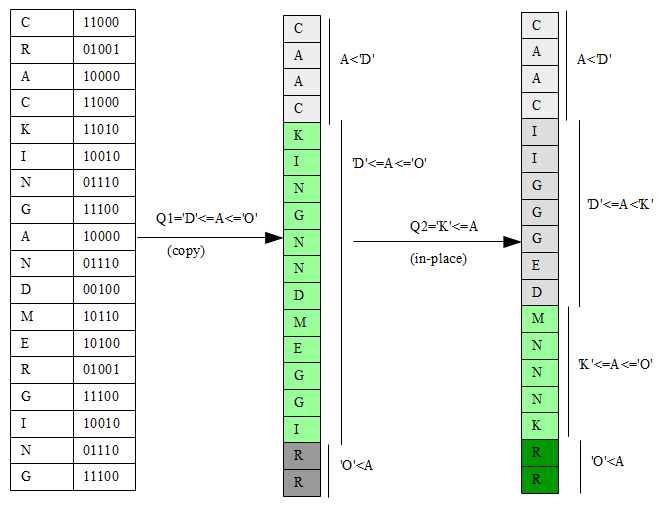
\includegraphics[width=\linewidth, height=5cm, keepaspectratio]{graphics/cracking.png}
\caption{Cracking a column.}
\end{figure}
\end{frame}

\subsection{Adaptive Merging}
\begin{frame}
\frametitle{Adaptive Merging}
\textbf{Main Idea: }incrementally merge sort the relevant key ranges till a single sorted partition is created. \pause
\begin{figure}
\centering
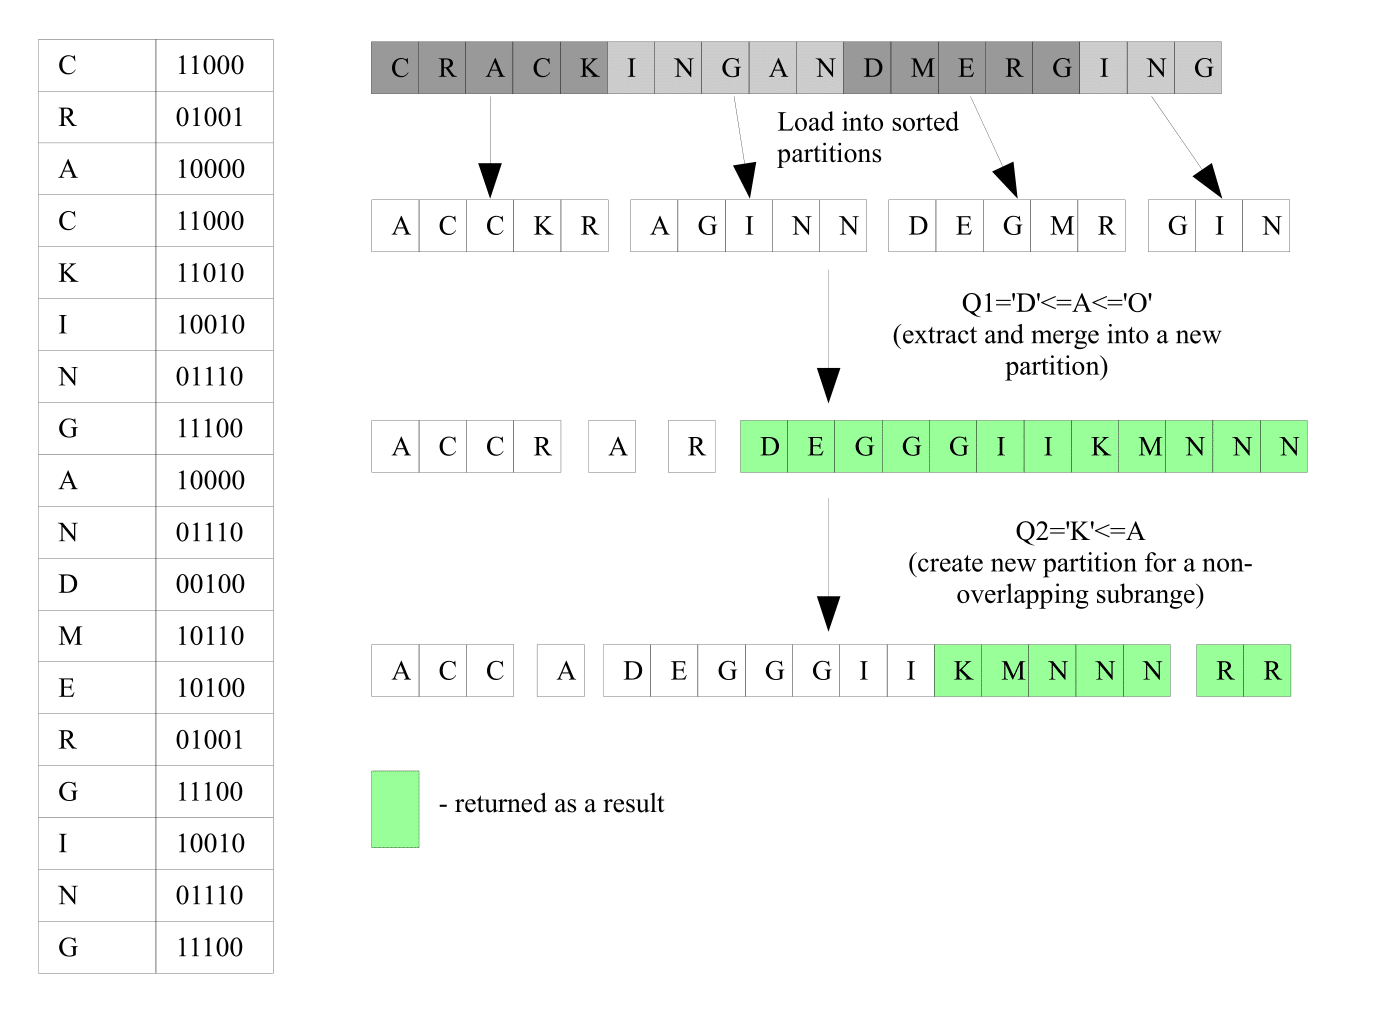
\includegraphics[width=\linewidth, height=5cm, keepaspectratio]{graphics/merging.png}
\caption{Example for adaptive merging.}
\end{figure}
\end{frame}

\subsection{Hybrid Approaches}
\begin{frame}
\frametitle{Database Cracking vs. Adaptive Merging}
\begin{tabular}{| M{0.2\linewidth} | }
\hline 
  \\ 
\hline 
\textbf{Initial Run} \\ 
\hline 
\textbf{Response Time} \\ 
\hline 
\textbf{Convergence} \\ 
\hline 
\end{tabular} 
\end{frame}

\begin{frame}
\frametitle{Database Cracking vs. Adaptive Merging}
\begin{tabular}{| M{0.2\linewidth} | M{0.35\linewidth} |}
\hline 
 & \textbf{Database Cracking} \\ 
\hline 
\textbf{Initial Run} & \color{green} slightly slower than scan \\ 
\hline 
\textbf{Response Time} & \color{green} faster than scan after 1$^{st}$ query \\ 
\hline 
\textbf{Convergence} & \color{red} after 1k queries, 40\% slower than full index  \\ 
\hline 
\end{tabular} 
\end{frame}

\begin{frame}
\frametitle{Database Cracking vs. Adaptive Merging \footnote{experimental data taken from [5]}}
\begin{tabular}{| M{0.2\linewidth} | M{0.35\linewidth} | M{0.35\linewidth} |}
\hline 
 & \textbf{Database Cracking} & \textbf{Adaptive Merging} \\ 
\hline 
\textbf{Initial Run} & \color{green} slightly slower than scan & \color{red} approx. 5 times slower than scan \\ 
\hline 
\textbf{Response Time} & \color{green} faster than scan after 1$^{st}$ query & \color{red} first queries are slower than scan \\ 
\hline 
\textbf{Convergence} & \color{red} after 1k queries, 40\% slower than full index & \color{green} 10M records $\Rightarrow$ approx. 40 queries \\ 
\hline 
\end{tabular} 
\end{frame}

\begin{frame}
\frametitle{Hybrid Approaches}
\textbf{Strategy} \pause
\begin{enumerate}
\item{Find the general structure:}
\begin{itemize}
\item{load data into partitions;}
\item{extract relevant data from each partition (\textit{crack});}
\item{load data into final partitions.}
\end{itemize}
\pause
\item{How to make components better?}
\begin{itemize}
\item{Crack;}
\item{Sort;}
\item{Radix.}
\end{itemize}
\pause
\item{Combine the best components}
\begin{itemize}
\item{Sort-*;}
\item{Crack-*;}
\item{Radix-*.}
\end{itemize}
\end{enumerate}
\end{frame}

\begin{frame}
\frametitle{Crack-Sort Algorithm}
\begin{figure}
\centering
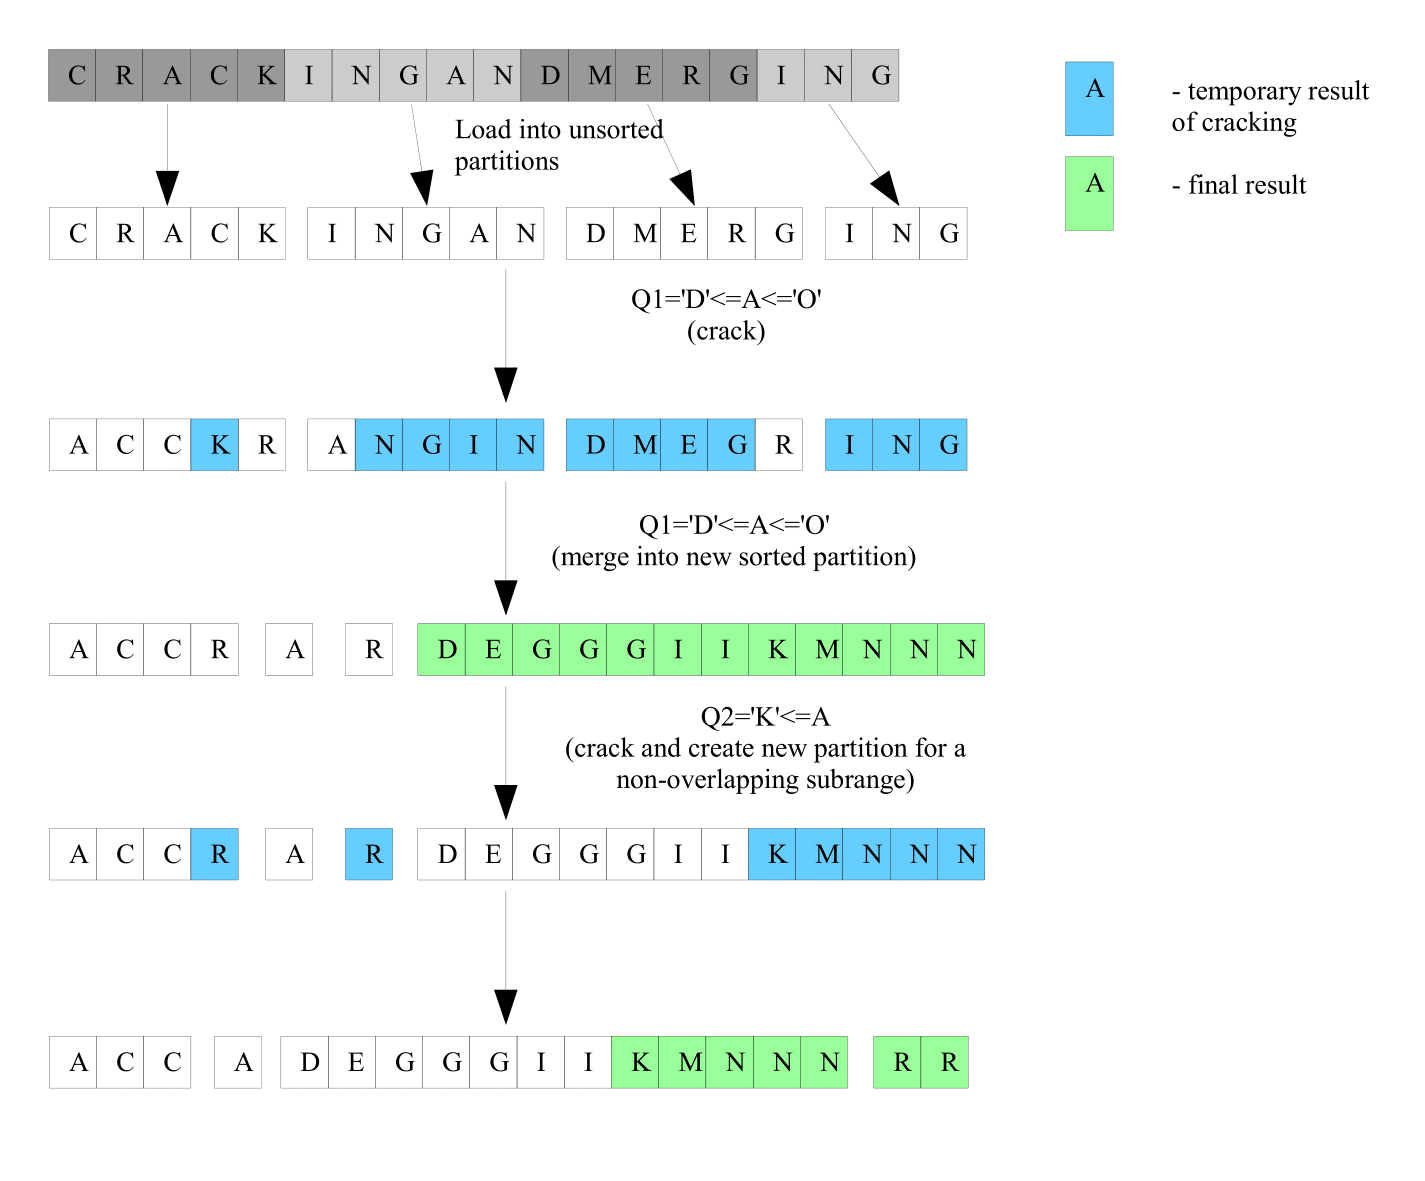
\includegraphics[height=6cm , keepaspectratio]{graphics/hcs.png}
\caption{Hybrid Crack-Sort Algorithm.}
\end{figure}

\end{frame}

\begin{frame}
\frametitle{Radix-Radix Algorithm}
\begin{figure}
\centering
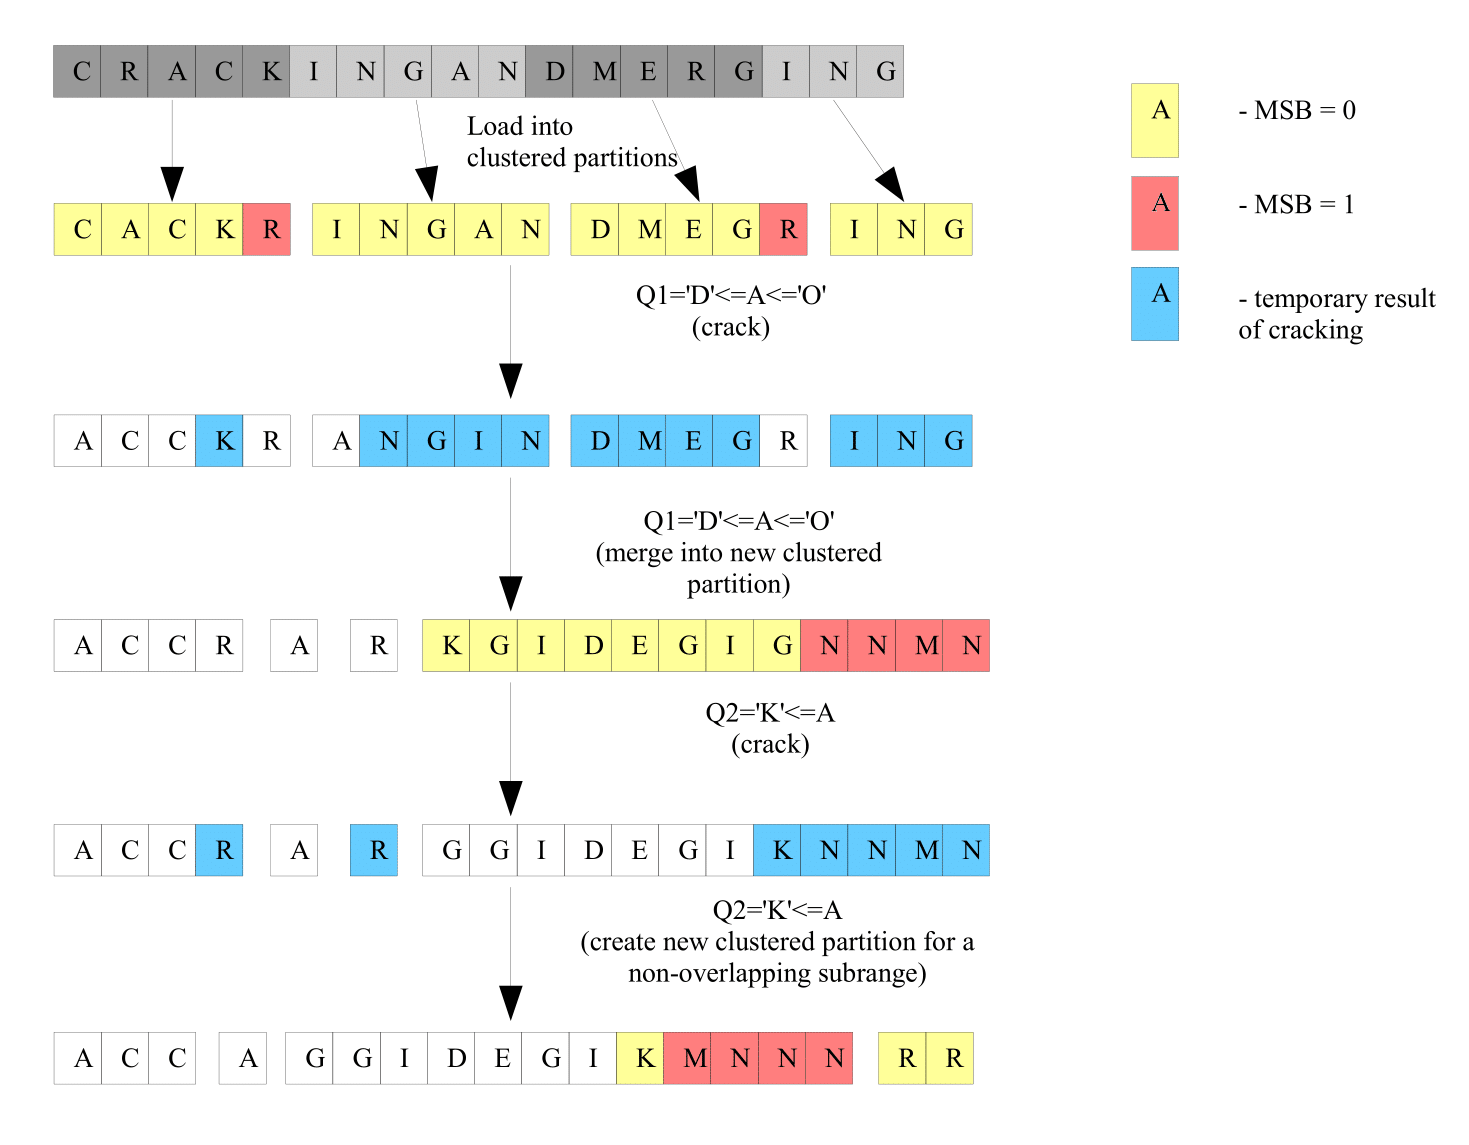
\includegraphics[height=6cm , keepaspectratio]{graphics/hrr.png}
\caption{Hybrid Radix-Radix Algorithm.}
\end{figure}
\end{frame}

\section{Lessons Learned}
\begin{frame}
\frametitle{Lessons Learned}
\begin{itemize}
\item{Adaptive Indexing Is a Promising Concept;}
\item{Database Cracking and Adaptive Merging Have Similar Nature;}\item{Crack-Sort and Crack-Radix Are Promising Alternatives;}
\item{Hybrid Algorithms Can Be Further Combined.}
\end{itemize}
\end{frame}

\section{Future Work}
\begin{frame}
\frametitle{Future Work}
\begin{itemize}
\item{Further Research on Adaptive Merging and Hybrid Approaches Needed;}
\item{New Strategies for Hybrid Algorithms;}
\item{Influence of Underlying Data Structure;}
\item{Integration of Adaptive Indexing into Other Models;}
\item{Extensions to the Methods.}
\end{itemize}
\end{frame}

\begin{frame}
\frametitle{Thank you for your attention!}
\end{frame}

\begin{frame}
\frametitle{Questions? Recommendations? Remarks?}
\end{frame}

\begin{frame}
\frametitle{Literature}
\begin{enumerate}
\item{Seshadri, Praveen, and Arun Swami. ”Generalized partial indexes.” Data Engineering, 1995. Proceedings of the Eleventh International Conference on. IEEE, 1995.}
\item{L\"uhring, Martin, et al. ”Autonomous management of soft indexes.” Data Engineering}
\item{Idreos, Stratos, Martin L. Kersten, and Stefan Manegold. ”Database
Cracking.” CIDR. Vol. 7. 2007.}
\item{Graefe, Goetz, and Harumi Kuno. ”Self-selecting, self-tuning, incrementally optimized indexes.” Proceedings of the 13th International Conference on Extending Database Technology. ACM, 2010.}
\item{Idreos, Stratos, et al. ”Merging what’s cracked, cracking what’s merged: adaptive indexing in main-memory column-stores.” Proceedings of the VLDB Endowment 4.9, 2011.}
\end{enumerate}
\end{frame}


\end{document}
